\documentclass[draft,linenumbers]{agujournal}
\draftfalse
\usepackage{hyperref}
\usepackage[export]{adjustbox}
\addtolength{\oddsidemargin}{-.875in}
\addtolength{\evensidemargin}{-.875in}
	
\hypersetup{
    colorlinks=true,
    linkcolor=blue,
    filecolor=magenta,      
    urlcolor=cyan,
}

\journalname{Journal of Advances in Modeling Earth Systems (JAMES)}

\begin{document}

 \begin{figure}[h]
    % \centering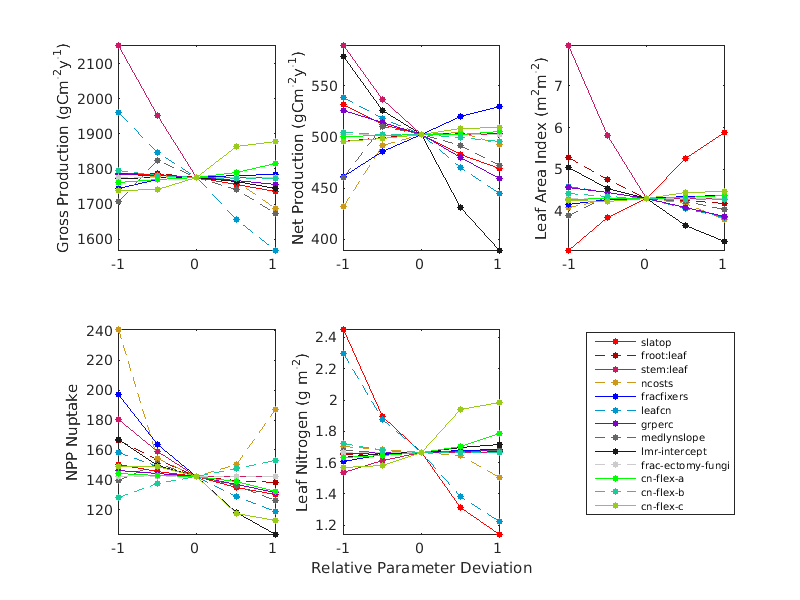
\includegraphics[width=0.5\textwidth, right]{lion-lo9
     \includegraphics[width=1.3\textwidth, left]{matlab/figures/frac_deviation_p1CLM5_CAX__y1.png}
     \caption{Caxiuana State Parameter Sensitivity}
     \label{CAX state}
  \end{figure}
  
   \begin{figure}[h]
     \centering
     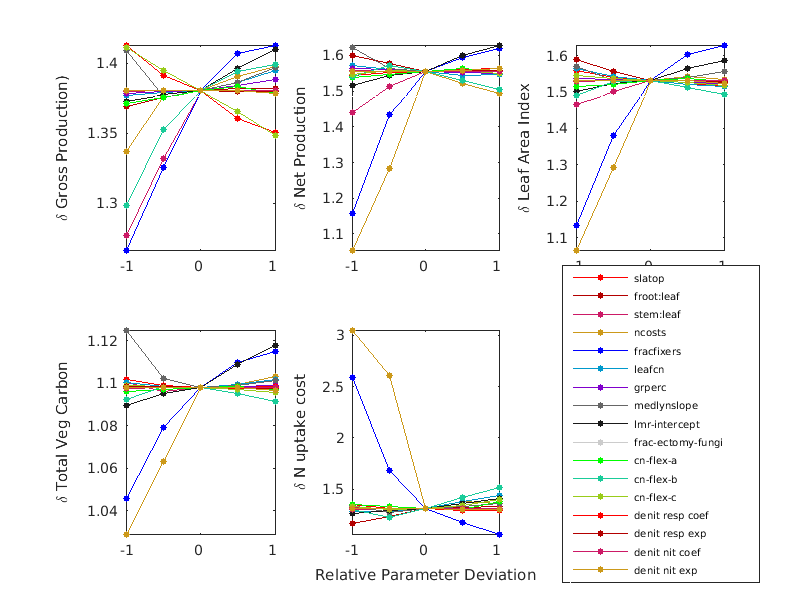
\includegraphics[width=1.3\textwidth, left]{matlab/figures/frac_deviation_p1CLM5_BCI__y1.png}
     \caption{BCI State Parameter Sensitivity}
     \label{BCI state}
  \end{figure}
  
 \begin{figure}[h]
     \centering
     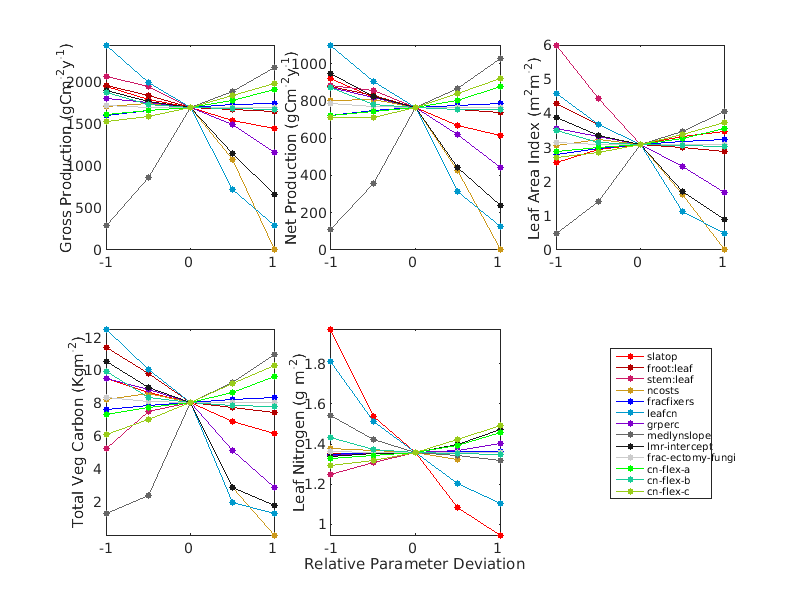
\includegraphics[width=1.3\textwidth, left]{matlab/figures/frac_deviation_p1CLM5_ORN__y1.png}
     \caption{Oak Ridge State Parameter Sensitivity}
     \label{ORN state}
  \end{figure}
  
  
 \begin{figure}[h]
     \centering
     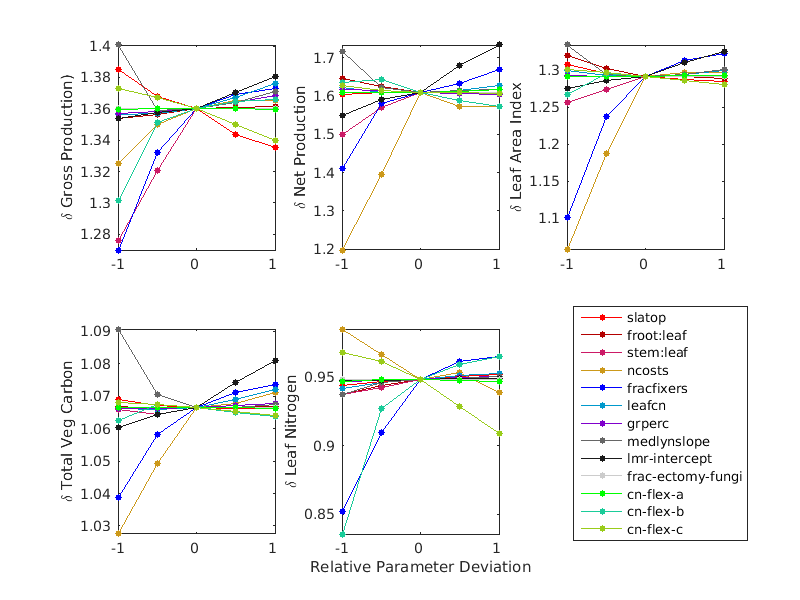
\includegraphics[width=1.3\textwidth, left]{matlab/figures/frac_deviation_CO2_response_1CLM5_1x1pt_Br-cax_ens_transient_ELEV_PI_y1.png}
     \caption{Caxiuana CO2 response}
     \label{Caxiuana CO2 response Parameter Sensitivity }
  \end{figure}
  
  
 \begin{figure}[h]
     \centering
     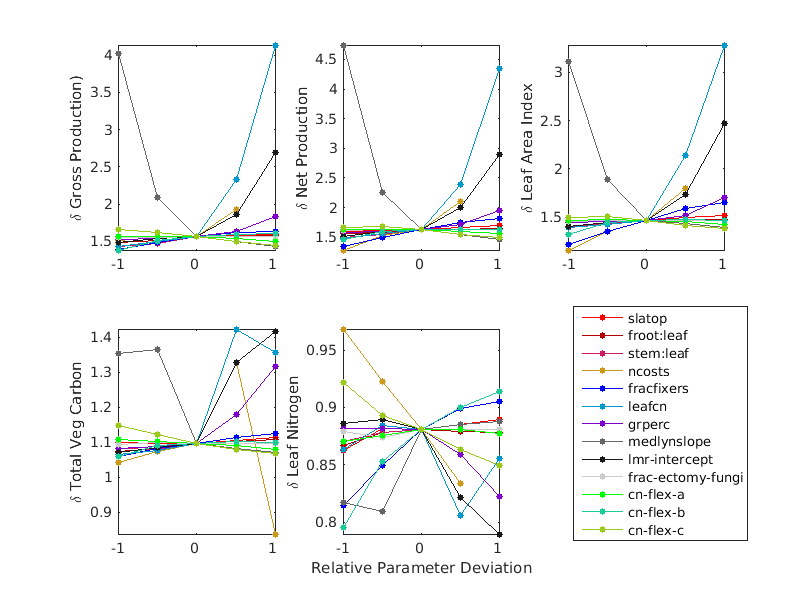
\includegraphics[width=1.3\textwidth, left]{matlab/figures/frac_deviation_CO2_response_1CLM5_1x1pt_US-ORN_ens_transient_ELEV_PI_y1.png}
     \caption{Oak Ridge CO2 response}
     \label{Oak Ridge CO2 response Parameter Sensitivity}
  \end{figure}
  

  
 \begin{figure}[h]
     \centering
     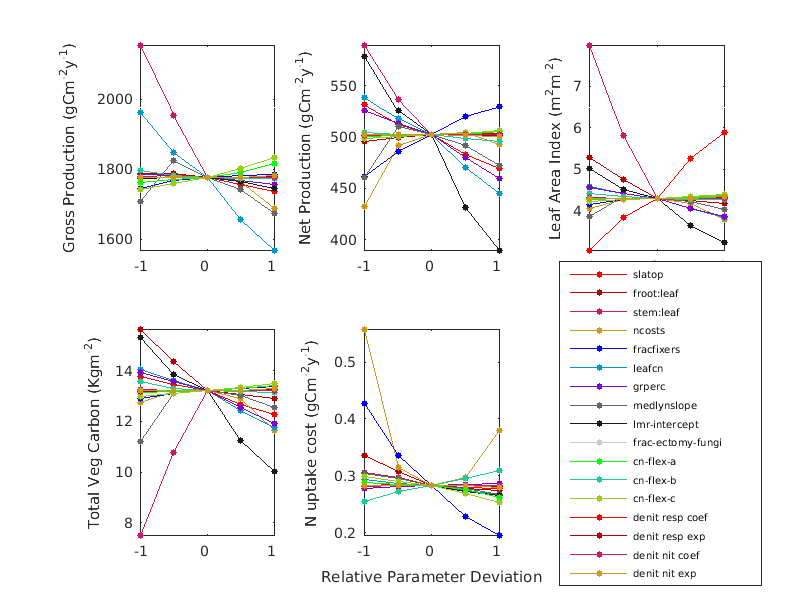
\includegraphics[width=1.3\textwidth, left]{matlab/figures/frac_deviation_CO2_response_1CLM5_BCI__y1.png}
     \caption{BCI CO2 response}
     \label{BCI CO2 response Parameter Sensitivity}
  \end{figure}
  
      
 \begin{figure}[h]
     \centering
     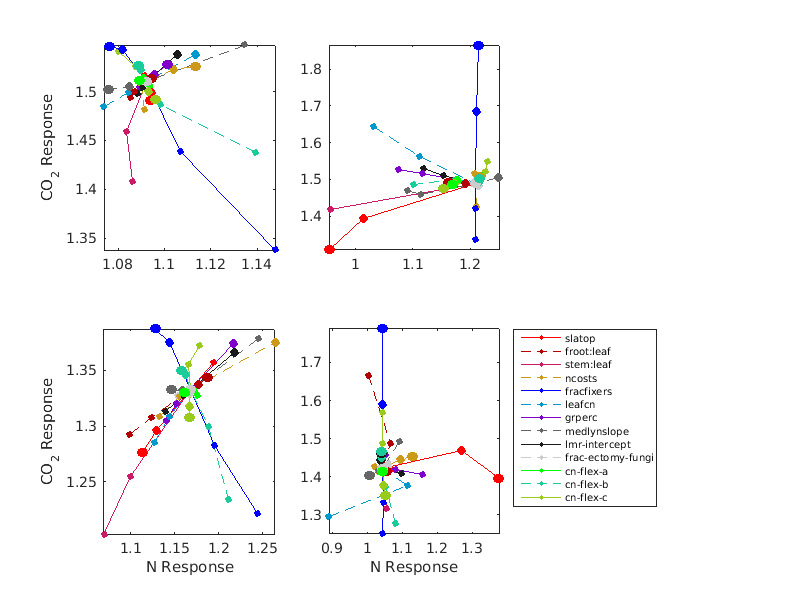
\includegraphics[width=1.55\textwidth, left]{matlab/figures/OCT_CNdep_GPP1_CLM50defpft_ndep_1x1pt_US-Me2_ens_MIC_p2006.png}
     \caption{GPP CO2 and N respones}
     \label{GPP CO2 and N respones}
  \end{figure}
  
      

\begin{figure}[h]
     \centering
     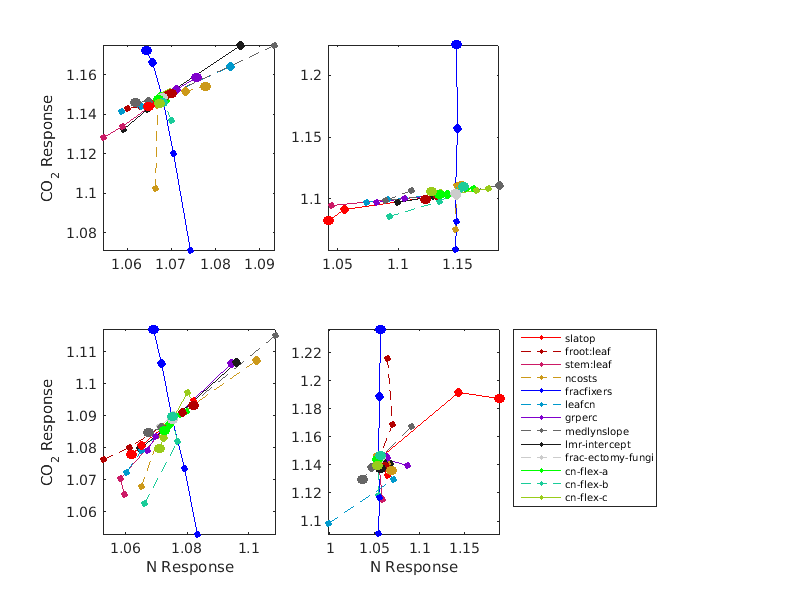
\includegraphics[width=1.55\textwidth, left]{matlab/figures/OCT_CNdep_TOTVEGC1_CLM50defpft_ndep_1x1pt_US-Me2_ens_MIC_p2006.png}
     \caption{Total vegetation carbon CO2 and N respones}
     \label{Total vegetation carbon CO2 and N respones}
  \end{figure}  
  
\end{document}